\documentclass[journal,12pt,twocolumn]{IEEEtran}
%
\usepackage{setspace}
\usepackage{gensymb}
%\doublespacing
\singlespacing

\usepackage{graphicx}
\graphicspath{{./fig/}}
%\usepackage{amssymb}
%\usepackage{relsize}
\usepackage[cmex10]{amsmath}
%\usepackage{amsthm}
%\interdisplaylinepenalty=2500
%\savesymbol{iint}
%\usepackage{txfonts}
%\restoresymbol{TXF}{iint}
%\usepackage{wasysym}
\usepackage{amsthm}
%\usepackage{iithtlc}
\usepackage{mathrsfs}
\usepackage{txfonts}
\usepackage{stfloats}
\usepackage{bm}
\usepackage{cite}
\usepackage{cases}
\usepackage{subfig}
%\usepackage{xtab}
\usepackage{longtable}
\usepackage{multirow}
%\usepackage{algorithm}
%\usepackage{algpseudocode}
\usepackage{enumitem}
\usepackage{mathtools}
\usepackage{steinmetz}
\usepackage{tikz}
\usepackage{circuitikz}
\usepackage{verbatim}
\usepackage{tfrupee}
\usepackage{inputenc}
%\usepackage[breaklinks=true]{hyperref}
\usepackage[hidelinks]{hyperref}
%\usepackage{stmaryrd}
\usepackage{tkz-euclide} % loads  TikZ and tkz-base
%\usetkzobj{all}
\usetikzlibrary{calc,math}
\usepackage{listings}
    \usepackage{color}                                            %%
    \usepackage{array}                                            %%
    \usepackage{longtable}                                        %%
    \usepackage{calc}                                             %%
    \usepackage{multirow}                                         %%
    \usepackage{hhline}                                           %%
    \usepackage{ifthen}                                           %%
  %optionally (for landscape tables embedded in another document): %%
    \usepackage{lscape}     
\usepackage{multicol}
\usepackage{chngcntr}
%\usepackage{enumerate}
%\usepackage{wasysym}
%\newcounter{MYtempeqncnt}
\DeclareMathOperator*{\Res}{Res}
%\renewcommand{\baselinestretch}{2}
\renewcommand\thesection{\arabic{section}}
\renewcommand\thesubsection{\thesection.\arabic{subsection}}
\renewcommand\thesubsubsection{\thesubsection.\arabic{subsubsection}}

\renewcommand\thesectiondis{\arabic{section}}
\renewcommand\thesubsectiondis{\thesectiondis.\arabic{subsection}}
\renewcommand\thesubsubsectiondis{\thesubsectiondis.\arabic{subsubsection}}

% correct bad hyphenation here
\def\inputGnumericTable{}                                 %%

\lstset{
%language=C,
frame=single, 
breaklines=true,
columns=fullflexible
}
%\lstset{
%language=tex,
%frame=single, 
%breaklines=true
%}

\begin{document}
%


\newtheorem{theorem}{Theorem}[section]
\newtheorem{problem}{Problem}
\newtheorem{proposition}{Proposition}[section]
\newtheorem{lemma}{Lemma}[section]
\newtheorem{corollary}[theorem]{Corollary}
\newtheorem{example}{Example}[section]
\newtheorem{definition}[problem]{Definition}
%\newtheorem{thm}{Theorem}[section] 
%\newtheorem{defn}[thm]{Definition}
%\newtheorem{algorithm}{Algorithm}[section]
%\newtheorem{cor}{Corollary}
\newcommand{\BEQA}{\begin{eqnarray}}
\newcommand{\EEQA}{\end{eqnarray}}
\newcommand{\define}{\stackrel{\triangle}{=}}
\bibliographystyle{IEEEtran}
%\bibliographystyle{ieeetr}
\providecommand{\mbf}{\mathbf}
\providecommand{\pr}[1]{\ensuremath{\Pr\left(#1\right)}}
\providecommand{\qfunc}[1]{\ensuremath{Q\left(#1\right)}}
\providecommand{\sbrak}[1]{\ensuremath{{}\left[#1\right]}}
\providecommand{\lsbrak}[1]{\ensuremath{{}\left[#1\right.}}
\providecommand{\rsbrak}[1]{\ensuremath{{}\left.#1\right]}}
\providecommand{\brak}[1]{\ensuremath{\left(#1\right)}}
\providecommand{\lbrak}[1]{\ensuremath{\left(#1\right.}}
\providecommand{\rbrak}[1]{\ensuremath{\left.#1\right)}}
\providecommand{\cbrak}[1]{\ensuremath{\left\{#1\right\}}}
\providecommand{\lcbrak}[1]{\ensuremath{\left\{#1\right.}}
\providecommand{\rcbrak}[1]{\ensuremath{\left.#1\right\}}}
\theoremstyle{remark}
\newtheorem{rem}{Remark}
\newcommand{\sgn}{\mathop{\mathrm{sgn}}}
\providecommand{\abs}[1]{\left\vert#1\right\vert}
\providecommand{\res}[1]{\Res\displaylimits_{#1}} 
\providecommand{\norm}[1]{\left\lVert#1\right\rVert}
%\providecommand{\norm}[1]{\lVert#1\rVert}
\providecommand{\mtx}[1]{\mathbf{#1}}
\providecommand{\mean}[1]{E\left[ #1 \right]}
\providecommand{\fourier}{\overset{\mathcal{F}}{ \rightleftharpoons}}
%\providecommand{\hilbert}{\overset{\mathcal{H}}{ \rightleftharpoons}}
\providecommand{\system}{\overset{\mathcal{H}}{ \longleftrightarrow}}
	%\newcommand{\solution}[2]{\textbf{Solution:}{#1}}
\newcommand{\solution}{\noindent \textbf{Solution: }}
\newcommand{\cosec}{\,\text{cosec}\,}
\providecommand{\dec}[2]{\ensuremath{\overset{#1}{\underset{#2}{\gtrless}}}}
\newcommand{\myvec}[1]{\ensuremath{\begin{pmatrix}#1\end{pmatrix}}}
\newcommand{\mydet}[1]{\ensuremath{\begin{vmatrix}#1\end{vmatrix}}}
%\numberwithin{equation}{section}
\numberwithin{equation}{subsection}
%\numberwithin{problem}{section}
%\numberwithin{definition}{section}
\makeatletter
\@addtoreset{figure}{problem}
\makeatother
\let\StandardTheFigure\thefigure
\let\vec\mathbf
%\renewcommand{\thefigure}{\theproblem.\arabic{figure}}
%\renewcommand{\thefigure}{\theproblem}
%\setlist[enumerate,1]{before=\renewcommand\theequation{\theenumi.\arabic{equation}}
%\counterwithin{equation}{enumi}
%\renewcommand{\theequation}{\arabic{subsection}.\arabic{equation}}
\def\putbox#1#2#3{\makebox[0in][l]{\makebox[#1][l]{}\raisebox{\baselineskip}[0in][0in]{\raisebox{#2}[0in][0in]{#3}}}}
     \def\rightbox#1{\makebox[0in][r]{#1}}
     \def\centbox#1{\makebox[0in]{#1}}
     \def\topbox#1{\raisebox{-\baselineskip}[0in][0in]{#1}}
     \def\midbox#1{\raisebox{-0.5\baselineskip}[0in][0in]{#1}}
\vspace{3cm}
\title{Model selection for Galactic Double Neutron Star total masses}
\author{PH6130 course project\\by\\Shreeprasad Bhat (AI20MTECH14011)\\M.Tech Artifical Intelligence\\IIT Hyderabad}
%\title{
%	\logo{Matrix Analysis through Octave}{\begin{center}\includegraphics[scale=.24]{tlc}\end{center}}{}{HAMDSP}
%}
% paper title
% can use linebreaks \\ within to get better formatting as desired
%\title{Matrix Analysis through Octave}
%
%
% author names and IEEE memberships
% note positions of commas and nonbreaking spaces ( ~ ) LaTeX will not break
% a structure at a ~ so this keeps an author's name from being broken across
% two lines.
% use \thanks{} to gain access to the first footnote area
% a separate \thanks must be used for each paragraph as LaTeX2e's \thanks
% was not built to handle multiple paragraphs
%
%\author{<-this % stops a space
%\thanks{}}
%}
% note the % following the last \IEEEmembership and also \thanks - 
% these prevent an unwanted space from occurring between the last author name
% and the end of the author line. i.e., if you had this:
% 
% \author{....lastname \thanks{...} \thanks{...} }
%                     ^------------^------------^----Do not want these spaces!
%
% a space would be appended to the last name and could cause every name on that
% line to be shifted left slightly. This is one of those "LaTeX things". For
% instance, "\textbf{A} \textbf{B}" will typeset as "A B" not "AB". To get
% "AB" then you have to do: "\textbf{A}\textbf{B}"
% \thanks is no different in this regard, so shield the last } of each \thanks
% that ends a line with a % and do not let a space in before the next \thanks.
% Spaces after \IEEEmembership other than the last one are OK (and needed) as
% you are supposed to have spaces between the names. For what it is worth,
% this is a minor point as most people would not even notice if the said evil
% space somehow managed to creep in.
% The paper headers
%\markboth{Journal of \LaTeX\ Class Files,~Vol.~6, No.~1, January~2007}%
%{Shell \MakeLowercase{\textit{et al.}}: Bare Demo of IEEEtran.cls for Journals}
% The only time the second header will appear is for the odd numbered pages
% after the title page when using the twoside option.
% 
% *** Note that you probably will NOT want to include the author's ***
% *** name in the headers of peer review papers.                   ***
% You can use \ifCLASSOPTIONpeerreview for conditional compilation here if
% you desire.
% If you want to put a publisher's ID mark on the page you can do it like
% this:
%\IEEEpubid{0000--0000/00\$00.00~\copyright~2007 IEEE}
% Remember, if you use this you must call \IEEEpubidadjcol in the second
% column for its text to clear the IEEEpubid mark.
% make the title area
\maketitle
\newpage
\bigskip
%\renewcommand{\thefigure}{\theenumi}
%\renewcommand{\thetable}{\theenumi}
%\renewcommand{\theequation}{\theenumi}
% IEEEtran.cls defaults to using nonbold math in the Abstract.
% This preserves the distinction between vectors and scalars. However,
% if the journal you are submitting to favors bold math in the abstract,
% then you can use LaTeX's standard command \boldmath at the very start
% of the abstract to achieve this. Many IEEE journals frown on math
% in the abstract anyway.
% Note that keywords are not normally used for peerreview papers.
%\begin{IEEEkeywords}
%Cooperative diversity, decode and forward, piecewise linear
%\end{IEEEkeywords}
% For peer review papers, you can put extra information on the cover
% page as needed:
% \ifCLASSOPTIONpeerreview
% \begin{center} \bfseries EDICS Category: 3-BBND \end{center}
% \fi
%
% For peerreview papers, this IEEEtran command inserts a page break and
% creates the second title. It will be ignored for other modes.
%\IEEEpeerreviewmaketitle
\begin{abstract}
In this project, we analyse the population of 15 known galactic Double Neutron Stars (DNSs) regarding the total masses of these systems. We fit the distribution of total masses for a single Gaussian distribution, two-component and three component Gaussian mixture model. Multiple statistical tests are performed for model selection. A pure likelihood ratio test prefers Gaussian mixture model with 3 components and than with two components, but for small datasets this test can encourage over-fitting. This can be avoided by penalizing models with higher number of free parameters. Several simple and well established statistical test, including including information criteria (AICc, BIC), cross-validation and Bayesian evidence ratios are tried. We conclude that even-though a two and three-component mixture is consistent with the data, the model selection criteria consistently indicate that there is no robust preference for it over a single-component fit.\end{abstract}
\tableofcontents
\section{Reference}
Keitel, D., 2019. Galactic double neutron star total masses and Gaussian mixture model selection. Monthly Notices of the Royal Astronomical Society, 485(2), pp.1665-1674.
\section{Code}
Download the code from \textcolor{gray}{\url{https://github.com/shreeprasadbhat/data-science-project/blob/master/project.ipynb}}
\section{Introduction}
The population of galactic Double Neutron Stars (DNSs) or binary neutron stars (BNSs), as the gravitational wave (GW) community prefers to call them is of high interest as a locally accessible predictor for the population of merging binaries in the wider Universe, which has recently become accessible to GW observations with LIGO and Virgo. Traditionally, a lot of work has focused on using the observed galactic sample to predict coalescence rates, though the distribution of component masses has also been studied. Here we consider the total gravitational masses $M_{T}$ of 15 known DNSs. $M_{T}$ is of special interest in predicting the fate of binary merger remnants and for studies of the nuclear equation of state (EoS) point out an apparent bimodality in the distribution of $M_{T}$ , and with the help of Gaussian mixture models and different statistical test and caution against relying on likelihood-ratio tests alone, especially when applied to small data sets. First, for completeness, (i) visual inspection of the data set and (ii) GMM fitting and likelihood-ratio tests are briefly summarised. The additional hypothesis test methods include (iii) information criteria (AICc and BIC) that penalise under constrained parameters, (iv) a cross-validation test to understand the impact of individual DNS systems on model selection, (v) Bayesian evidence computation through nested sampling.
\section{Data set and visual inspection}
\begin{figure}[h]
\centering
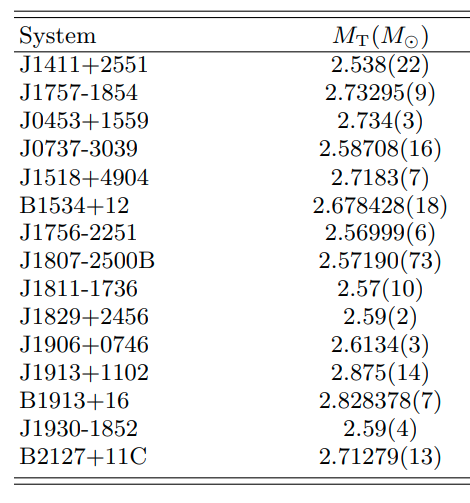
\includegraphics[scale=0.5]{fig/data_screenshot.png}
\caption{Dataset}
\end{figure}
Histograms of the $M_T$ data set are shown in Fig. 2. It compares the  the data by binning into $12$ bins and $24$ bins. Visually, $N_{bins} = 12$ makes a two-component fit appealing, while $N_{bins} = 24$ might even tempt the viewer into fitting three components. Note that the total number of data points is only $15$.
\begin{figure*}[h]
\centering
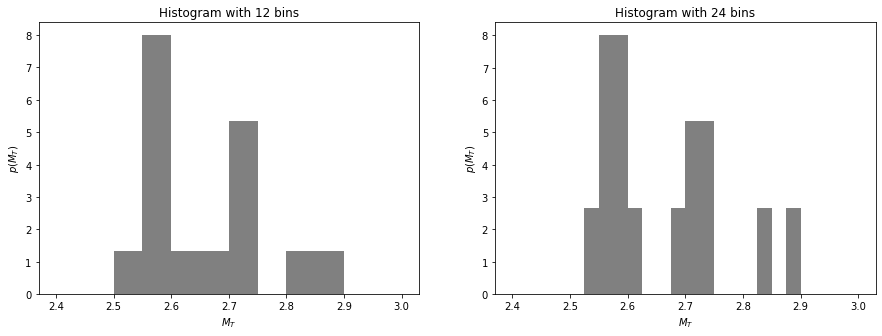
\includegraphics[width=\textwidth]{fig/hist.png}
\caption{Histogram of the total masses $M_T$}
\end{figure*}
\section{Modelling}
To probe possible structure in the $M_T$ distribution, below we fit the data with a Gaussian distribution model, a double Gaussian distribution model and triple Gaussian distribution model, respectively. 

The probability distribution function of Gaussian distribution model is given by
\begin{equation}
P\left(M_{T}, M_{0}, \sigma_{0}\right) = \frac{1}{\sqrt{2\pi}\sigma_{0}}exp\left(-\frac{(M_T-M_0)^2}{2\sigma_{0}^2}\right)
\end{equation}
and the best fit model from maximum likelihood estimate(MLE) is shown in Fig 3. and corresponding parameters are $(M_0, \sigma_0)=(2.67, 0.10).$
\begin{figure}[ht!]
\centering
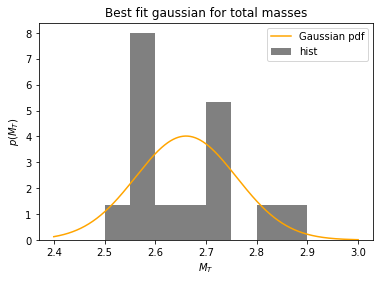
\includegraphics[scale=0.6]{fig/gau.png}
\caption{Best fit Gaussian for $M_T$}
\end{figure}

For the double Gaussian distribution model we have
\begin{multline}
P\left(M_{T}, M_{1}, M_{2}, \sigma_{1}, \sigma_{2}, C\right)\\ = \frac{C}{\sqrt{2\pi}\sigma_{1}}exp\left(-\frac{(M_T-M_1)^2}{2\sigma_{1}^2}\right)\\ + \frac{1-C}{\sqrt{2\pi}\sigma_{2}}exp\left(-\frac{(M_T-M_2)^2}{2\sigma_{2}^2}\right) 
\end{multline}
where $M_0(M_1, M_2)$, $\sigma_0(\sigma_1, \sigma_2)$ represent the mean and the variance of a Gaussian mass distribution, respectively, and C is defined as a weight of the first component. The best fit results from MLE are shown in Fig. 4, and the corresponding parameters are $(M_1 , \sigma_1) = (2.58, 0.01), (M_2 , \sigma_2) = (2.72, 0.08)$, and $C = 0.40$.
\begin{figure}[ht!]
\centering
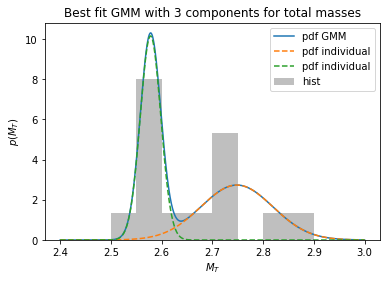
\includegraphics[scale=0.6]{fig/gmm2.png}
\caption{Best fit GMM, $N_{comp}=2$ for $M_T$}
\end{figure}

Similary, for the triple Gaussian distribution model we have
\begin{multline}
P\left(M_{T}, M_{1}, M_{2}, M_{3}, \sigma_{1}, \sigma_{2}, \sigma_{3}, C_1, C_2\right)\\ = \frac{C_1}{\sqrt{2\pi}\sigma_{1}}exp\left(-\frac{(M_T-M_1)^2}{2\sigma_{1}^2}\right)\\ + \frac{C_2}{\sqrt{2\pi}\sigma_{2}}exp\left(-\frac{(M_T-M_2)^2}{2\sigma_{2}^2}\right)\\+\frac{1-C_1-C_2}{\sqrt{2\pi}\sigma_{3}}exp\left(-\frac{(M_T-M_3)^2}{2\sigma_{3}^2}\right) 
\end{multline}
where $M_0(M_1, M_2, M_3)$, $\sigma_0(\sigma_1, \sigma_2, \sigma_3)$ represent the mean and the variance of a Gaussian mass distribution, respectively, and $C_1$, $C_2$ is defined as a weight of the first component. The best fit results from MLE are shown in Fig. 5.
\begin{figure}[ht!]
\centering
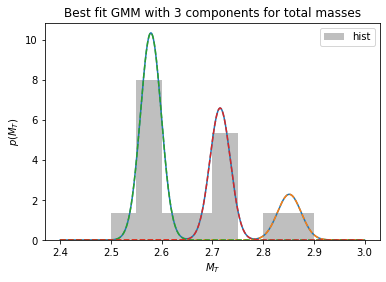
\includegraphics[scale=0.6]{fig/gmm3.png}
\caption{Best fit GMM, $N_{comp}=3$ for $M_T$}
\end{figure}
\section{Likelihood ratio test}
To evaluate the significance of the presence of a structure in the $M_T$ distribution (i.e., it consists of double Gaussian components rather than a single Gaussian component) we adopt the generalized likelihood ratio test that is widely used in hypothesis testing. Our null hypothesis is the single Gaussian distribution, and the alternative hypothesis is a double Gaussian $M_T$ distribution. We construct the likelihood ratio first, as the mass measurement of each neutron star is independent of others. The likelihood function is simply the product of probability for each independent measured total mass, i.e.,
\begin{equation}
	L(M_i, \sigma_i|x,M) = \prod_j P(x_j|M_i, \sigma_i;M)
\end{equation}
where $M_i$ , $\sigma_i$ are the fitting parameters, M represents the model we used, and $x_j$ represents the data. 

For $N_{data}$ data points $x_n$, the basic likelihood function for a GMM with $N_{comp}$ means $\mu_k$, with $\sigma_k$ and component weights $C_k \in [0,1]$
\begin{equation}
	L(x_n | {\mu_k, \sigma_k, C_k}) = \displaystyle\sum_{k=1}^{N_{comp}} \frac{C_k}{\sqrt{2\pi} \sigma_k} exp\left( -\frac{(x_n - \mu_k)^2}  {2\sigma_k^2}\right)
\end{equation}

And the likelihood ratio of single component Gaussian mixture to the double component Gaussian mixture is
\begin{equation}
	L_1 / L_2 = 0.0044
\end{equation}

And the likelihood ratio of double component Gaussian mixture to the triple component Gaussian mixture is
\begin{equation}
	L_2 / L_3 = 0.03
\end{equation}
\section{Information criteria: AICc and BIC}
In general, when adding additional components to a GMM the model likelihood will keep increasing. Hence, this test alone can tempt into overfitting any given data set. A more robust way of model selection is provided by information criteria which introduce a penalty term for higher numbers $N_{coeffs}$ of coefficients.
The Akaike Information Criterion (AIC) is given in its modified form as
\begin{equation}
	AICc = -2\ln L + 2N_{coeffs} + \frac{2 N_{coeffs} \left(N_{coeffs + 1}\right)}{N_{data}-N_{coeffs}-1}
\end{equation}
Here the second term is the original Akaike penalty for complex models, and the third term is a correction to produce more reliable rankings when N data is small. (The AICc converges to the original AIC for large N data) A popular alternative is the Bayesian Information Citerion (BIC):
\begin{equation}
	BIC = -2\ln L + N_{coeffs} \ln N_{data}
\end{equation}
The AICc and BIC computed for different Gaussian mixture model are
\begin{center}
\begin{tabular}{|c|c|c|}
\hline
& & \\
Likelihood ratio test & AICc & BIC\\
& & \\
\hline
GMM, $N_{comp} = 1$ & -21.71 & -21.29 \\
\hline
GMM, $N_{comp} = 2$ & -20.88 & -24.00 \\
\hline
GMM, $N_{comp} = 3$ & -4.54 & -22.88 \\
\hline
\end{tabular}
\end{center}
Despite its name, it is in general not equivalent to a full Bayesian evidence comparison between two models. Lower values of either criterion indicate a preferred model with a better balance between goodness-of-fit and parsimony. The strength of preference is given purely by the differences between models: any overall additive constant can be ignored. There is no universal agreement on how large a difference constitutes clear preference between models, though values between 3 and 5 are usually quoted. Note also that these criteria are formally motivated by asymptotic considerations which cannot be invoked for the small-N data problem under consideration here. Information criteria are generally expected to converge on a consistent answer when the data are indeed informative about the model selection question. Hence, it appears that for the $M_T$ distribution of Galactic DNS systems, the data set is simply not yet large (and/or precise) enough to conclusively answer the question.
\section{Cross-validation}
Another independent check for overfitting is cross-validation(CV). The basic idea is to check the intra-sample variance of a data set by re-evaluating fits on subsets of the data. For each iteration, a figure of merit (e.g. log-likelihood) is computed on the left-out data points, and in the end averaged over iterations. (In other words, for each iteration, the left-out data are a ‘test’ set for a model ‘trained’ on the remaining data.) Overly complex models are expected to get over-fit to the training subsets and then provide inferior prediction performance on the test subsets. The conceptually simplest version is leave-one-out CV, where all possible subsets of $N_{data}-1$ data points are exhaustively evaluated. Numerical cross-validation scores turn out not to be useful for this small data set, as the variance is too large to make any robust statements. However, an illustrative analysis in the spirit of leave-one-out CV is easily done by fitting GMMs for all 15 subsets of 14 data points each. This also helps identify systems that have a large effect on the fit. The individual fitted distributions for each iteration are compared in Fig. 3. When ignoring measurement errors, individual systems in the $M_T$ . 2.65M range have a large influence on the two-component fits, with the lower-mass peak sometimes even shifting to within the visually apparent ‘gap’.
\begin{figure}[ht!]
\centering
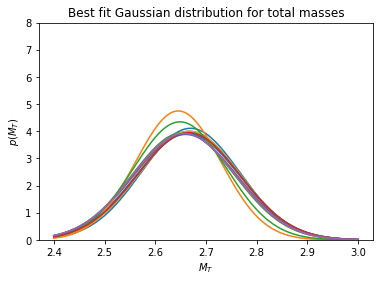
\includegraphics[scale=0.6]{fig/cv_gau.png}
\caption{Cross validation of Gaussian fit $M_T$}
\end{figure}
\begin{figure}[ht!]
\centering
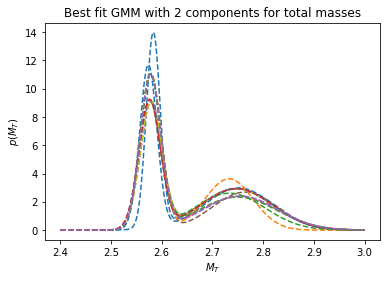
\includegraphics[scale=0.6]{fig/cv_gmm2.png}
\caption{Cross validation of GMM, $N_{comp}=2$}
\end{figure}
\begin{figure}[ht!]
\centering
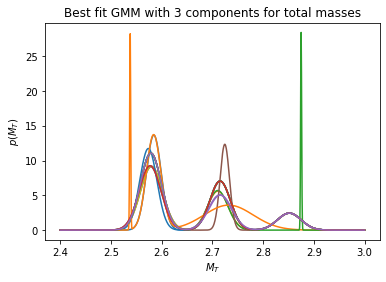
\includegraphics[scale=0.6]{fig/cv_gmm3.png}
\caption{Cross validation of GMM, $N_{comp}=3$}
\end{figure}
\section{Bayesian evidence}
Since the DNS data set is so small ($N_{data} = 15$), it is computationally cheap to obtain Bayesian posterior estimates and evidences for model selection. Starting from some prior knowledge $I$, a prior distribution $P(\theta | H,I)$ for the parameters $\theta$ of a model $H(\theta)$, and the GMM likelihood $P(x|\theta,H,I)=L(x_n|{\mu_k, \sigma_k, C_k})$, the posterior distribution for $\theta$ under that model follows from Bayes theorem:
\begin{equation}
	P(\theta|x,H,I) = \frac{P(\theta|H,I) P(x|\theta, H, I)}{P(x|H,I)}
\end{equation}
The Bayesian evidence for a model H is defined as its likelihood marginalised over its whole prior support,
\begin{equation}
	Z_H = P(x|H,I) = \int d\theta P(\theta|H,I) P(x|\theta,H,I)
\end{equation}
Note that this is still dependent on the model $H$, whereas the total evidence $P(x|I)$ would be a model-independent normalisation factor. Evidence ratios, also called Bayes factors, are a convenient quantity for model selection, as priors need to be defined only over the parameter space of each model, but not between models.
To evaluate $Z_H$ for GMMs of different $N$ comp , we can use CPNest, a python implementation of the nested sampling algorithm, with the likelihood function and $N_{live} = 1024$ sampler live points. The outcome of Bayesian inference in general depends on the choice of priors $P_(\theta| H,I);$ the following results are obtained from weakly informative priors. Overall, the CPNest posterior estimates and evidence ratios appear stable under reasonable prior changes.
CPNest results are also included in Table. 
\begin{center}
\begin{tabular}{|c|c|}
\hline
Model & log Z\\
\hline
GMM, $N_{comp}=1$ & 12.62 ± 0.012\\
\hline
GMM, $N_{comp}=2$ & -8.67 ± 0.05\\
\hline
\end{tabular}
\end{center}
The $N_{comp} = 1,2$ posteriors are also illustrated in Fig 9. and Fig 10. In addition, Fig shows the median reconstructed GMM distribution functions and their $90\%$ intervals. No CPNest likelihood point estimates are included in Table 1 since these might be misleading without context: Near the posterior median, $log_{10} L$ is generally close to the previous fit results, while higher values can be found in some overall less favoured parts of parameter space. The main quantity of interest for model comparison, the model evidence $Z_H$ , is not derived from a point estimate, but it takes into account the whole sampled volume. At $Z_2/Z_1 \leq 1.4, Z_2Z_3 \approx 1.1$, the evidence ratios are indecisive, meaning that the increased prior volume of GMMs with higher $N_{comp}$ just about makes up for the higher likelihoods achieved, and no clear preference for either model can be found. 
\begin{figure*}[ht!]
\centering
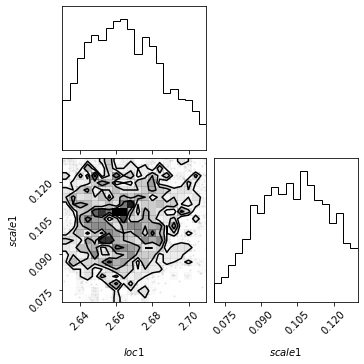
\includegraphics{fig/bay_evi_gau.png}
\caption{Corner plots for Gaussian fit}
\end{figure*}
\begin{figure*}[ht!]
\centering
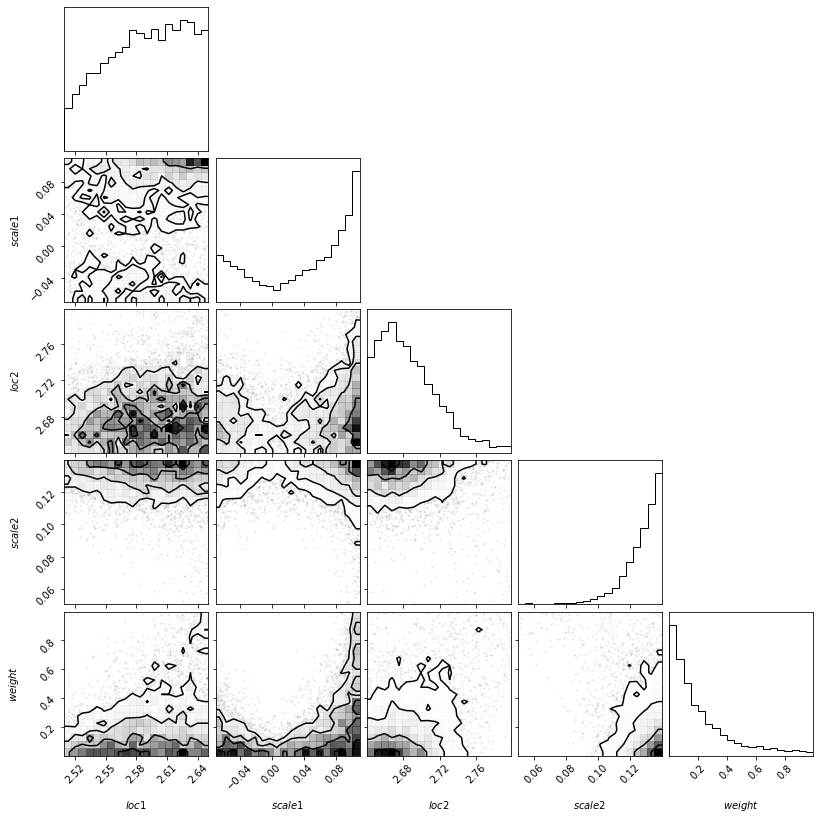
\includegraphics[width=\textwidth]{fig/bay_evi_gmm2.png}
\caption{Corner plots for GMM, $N_{comp}=2$}
\end{figure*}
\section{Conclusions}
The distribution of total masses $M_T$ of Galactic DNS systems shows can be fit into unimodal, bimodal or trimodal gaussian distribution. A pure likelihood ratio test prefers those two components over one, with estimating the significance of this preference as $2\sigma$. We have not considered measurement errors into account for any model fit. But considered more robust model selection criteria: Neither the frequentist information criteria (AICc and BIC) which amend the likelihood ratio test with a penalty for the higher number of free parameters in multi-component GMMs, nor a Bayesian evidence ratio test find any robust preference for more than one component. The various GMM fitting methods employed here still all agree with that a two component GMM certainly provides a good fit to the data; the scenario is not ruled out either, could have interesting consequences for stellar evolution models and GW astronomy. But it appears that the present set of known DNSs is simply too small, and some systems masses are not constrained well enough, to robustly decide between one or two components.
\end{document}
